\begin{savequote}[75mm]
The beginning is the most important part of the work.
\qauthor{Plato, The Republic}
\end{savequote}

% pending plagiarism check
\begin{flushleft}
\chapter{Establishing patient derived organoids for high-throughput image-based profiling}

Patient derived organoids can be established from diverse healthy or malignant tissues and have been shown to represent their tissue and tumor of origin with respect to morphologic and molecular features including gene expression and mutations \cite{Fujii:2016jo, Weeber2015-sn, Van_De_Wetering2015-ko, Sato:2011-1h,  Broutier2017-wg}. To generate personalized cancer models for phenotypic compound screening, I built a standardized clinical and laboratory workflow to generate patient derived organoids from patients with colorectal cancer using endoscopic biopsy samples (Figure 1a). Briefly, fresh patient samples were washed and digested and rembedded in a basal membrane extract. The medium, termed ENA, was based on Advanced DMEM/F12 (Life technologies) and supplemented with growth factors, including Epidermal Growth Factor (EGF), the BMP-signaling antagonist Noggin and the small-molecule TGF\beta-signaling inhibitor A83-01. 

\begin{figure}[h]
\centering
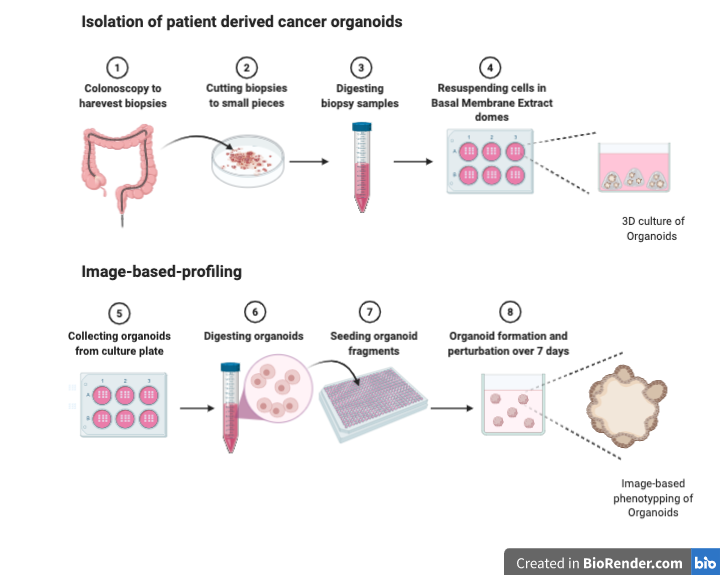
\includegraphics[scale=.35]{figures/organoid_establishment.png}
\caption{Organoid isolation and image-based profiling.}
\label{colon_cancer_progression}
\end{figure}

Patient derived organoids from 19 patients with colorectal cancer were prospectively developed. Donors to the biobank were representative of different clinical stages (Figure 1b, Supplemental Table S1). Gene expression profiling and amplicon sequencing of frequently altered genes colorectal cancer showed molecular profiles characteristic for colorectal cancer (Figure 1c-d). Similar to sequencing studies of primary tumors, we observed a high frequency of APC (47\%), KRAS (47\%) and TP53 (36\%) mutations in patient derived organoid cultures \cite{Muzny2012-hr} (Figure 1d, Supplemental Table S2). On a gene expression level, patient derived organoids mainly represented the canonical consensus molecular subtype CMS 2 of colorectal cancer \cite{Guinney2015-ex}. No patient derived organoid line with a MSI-high phenotype and the associated CMS 1 molecular subtype was established. Also, no organoid line matched the molecular subtype CMS 4, which is associated with stromal infiltration and TGF\beta-signaling. These observations are in line with previous observations \cite{Van_De_Wetering2015-ko, Schutte2017-fl} and the limitations of the organoid culture system, which (1) selects for growth of intestinal epithelial cells and their progeny and (2) uses small molecule inhibitors of TGF\beta-signaling to ensure organoid proliferation ex vivo \cite{Sato2011-lh}.

\begin{figure}[h]
\centering
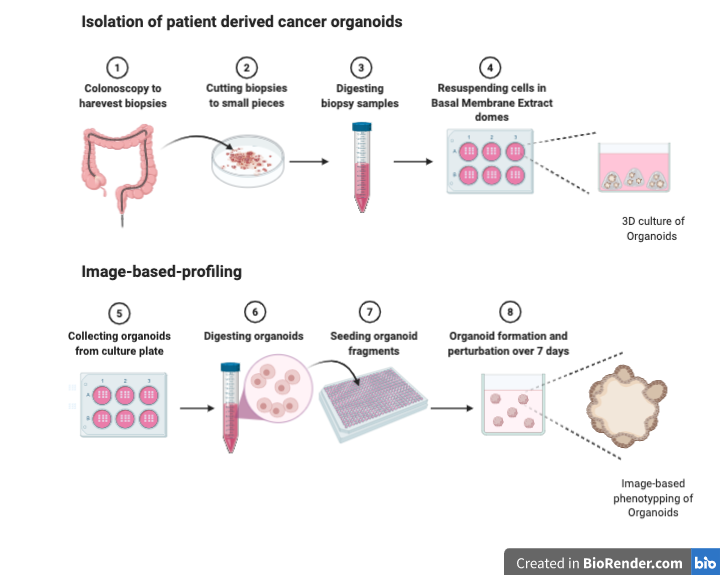
\includegraphics[scale=.35]{figures/organoid_establishment.png}
\caption{Organoid isolation and image-based profiling.}
\label{colon_cancer_progression}
\end{figure}

\end{flushleft}
